% !TeX spellcheck = en_US
% !TeX encoding = UTF-8
\section{Metadynamics\label{Sec:ES:metadynamics}}
Metadynamics, vividly called flooding method, was first suggested by Laio and Parrinello in 2002.\cite{LaioPNAS2002} 
%Imaging you became Doraemon in a dream. 
Imaging you were standing in a valley and were surrounded by high mountains. In most of the time, you were just wandering near the minimum, because your kinetic energy was not enough to climb the mountains. Suddenly, you realized that you could use metadynamics as a magic to escape from the minimum. You started walking. After each step, you took a bottle of sand out of your miraculous pocket and put the sand under your feet. Then you were lifted up inch-by-inch, and the deposited sand piles discourage you from revisiting where you had visited. And you were finally raised up to the top of the mountain and at that moment you were able to climb over that mountain without much effort and fell into another valley. The magic of sand continued, and at last you smoothed the whole area. Because you kept recording where you had put the sand and how much sand you had put there. You drew the shape the piled sand according to the record and you flipped it. In this way, you got the exact shape of the original free energy landscape up to a constant. 
\begin{figure}[htbp]
	\centering
	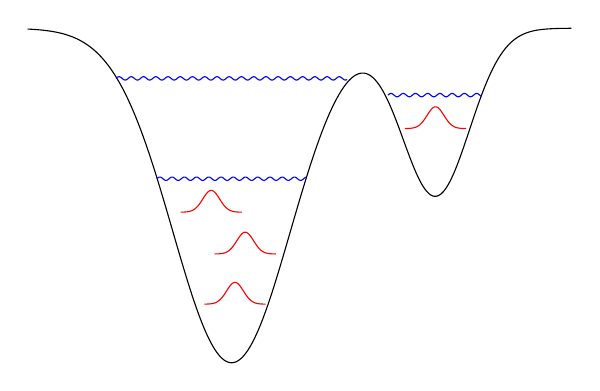
\begin{tikzpicture}
	\def\lims{xmin=-6,xmax=10,ymin=-2.1,ymax=0.01}
    \begin{axis}[\lims,hide x axis, hide y axis,width=0.7\textwidth,height=0.5\textwidth]
	    \addplot[mark=none,samples=1000,domain=-10:10,y domain=-2.1:0.01] {-2*exp(-x*x/6)-1*exp(-(x-6)*(x-6)/2)};
	    \addplot[red,mark=none,samples=1000,domain=-0.8:1.0] {-1.65+0.13*exp(-49*(x-0.1)*(x-0.1)/6)};
	    \addplot[red,mark=none,samples=1000,domain=-0.5:1.3] {-1.35+0.13*exp(-49*(x-0.4)*(x-0.4)/6)};
	    \addplot[red,mark=none,samples=1000,domain=-1.5:0.3] {-1.1+0.13*exp(-49*(x+0.6)*(x+0.6)/6)};
	    \addplot[blue,mark=none,samples=1000,domain=-2.2:2.2] {-0.9+0.01*sin(1000*(x+2.2))};
	    \addplot[blue,mark=none,samples=1000,domain=-3.4:3.4] {-0.3+0.01*sin(1000*(x+3.4))};
	    
	    \addplot[red,mark=none,samples=1000,domain=5.1:6.9] {-0.60+0.13*exp(-49*(x-6.0)*(x-6.0)/6)};
	    \addplot[blue,mark=none,samples=1000,domain=4.6:7.35] {-0.4+0.01*sin(1000*(x-4.6))};
	\end{axis}
	\end{tikzpicture}
	\caption{A schematic representation of metadynamics. The free energy well is gradually filled up with small Gaussians, and a transition is facilitated.}\label{Fig:ES:metadynamics}
\end{figure}

%\begin{figure}[htbp]
%	\centering
%	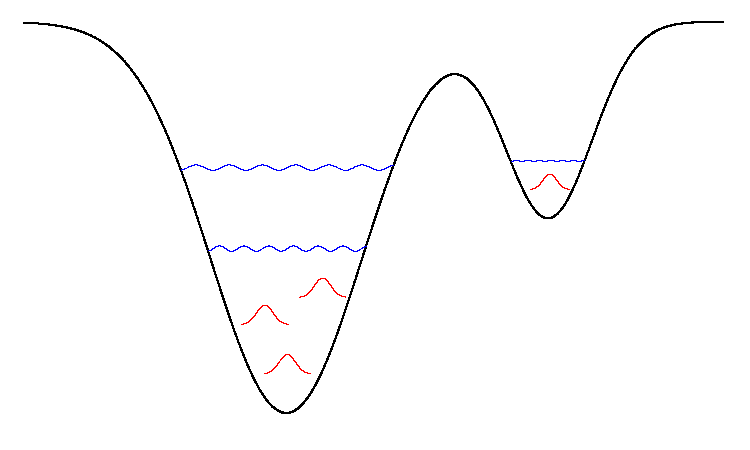
\includegraphics[width=0.8\textwidth]{figures/metadynamics.pdf}\\
%	\caption{A schematic representation of metadynamics. The free energy well is gradually filled up with small Gaussians, and a transition is facilitated.}\label{Fig:ES:metadynamics}
%\end{figure}

The above texts are merely an informal explanation of metadynamics. Formally, metadynamics belongs to a class of methods in which sampling is facilitated by introducing additional bias potential to pre-selected degrees of freedom, which are often referred as collective variables (CVs). In metadynamics, the bias potential added to the Hamiltonian of the system is history-dependent, and is often written as a sum of Gaussians deposited during the simulation as
\begin{equation}
   V_G(\mathbf{s},t) = \int\limits_0^t\diff t^\prime \omega\exp{\left(-\sum\limits_{i=1}^{d}\frac{\left[\mathbf{s}_i(R)-\mathbf{s}_i(R(t^\prime))\right]^2}{2\sigma_i^2}\right)}
\end{equation}
on a collective variable $\mathbf{s}$ in $d$-dimension. $\sigma$ and $\omega$ are two parameters tuning the shape of the Gaussians, which can be time-dependent. Asymptotically, 
\begin{equation}
   V_G(\mathbf{s},t\rightarrow \infty) = -G(\mathbf{s})+C.
\end{equation}

Recent improvement over the ordinary metadynamics on convergence issue, which is termed well-tempered metadynamics (WTMetaD), can be found in Ref.~\cite{BarducciPRL2008} and is reviewed in Ref.~\cite{ValssonARPC2016}. In this method, a gradually tempered Gaussian hill
\begin{equation}
    V_n(\mathbf{s})=V_{n-1}(\mathbf{s})+G(\mathbf{s},\mathbf{s}_n)\exp{\left[-\frac{1}{\gamma-1}\beta V_{n-1}(\mathbf{s}_n)\right]}
\end{equation}
is accumulated, where $V_0(\mathbf{s})=0$ and
\begin{equation}
    G(\mathbf{s},\mathbf{s}^\prime)=W\exp{\left(-||\mathbf{s}-\mathbf{s}^\prime||^2\right)}
\end{equation}
with $||\mathbf{s}-\mathbf{s}^\prime||^2$ being a distance metric such as
\begin{equation}
    ||\mathbf{s}-\mathbf{s}^\prime||^2=\frac{1}{2}\sum_{i,j}{(\mathbf{s}_i-\mathbf{s}_i^\prime)\Sigma_{i,j}^{-1}(\mathbf{s}_j-\mathbf{s}_j^\prime)}.
\end{equation}
$\Sigma_{i,j}^{-1}$ is the inverse of the covariance matrix $\Sigma_{i,j}$, and the latter is normally diagonal $\Sigma_{i,j}=\delta_{i,j}\sigma_i^2$. $W$ is the height of the Gaussian. $G(\mathbf{s},\mathbf{s}_n)$ is the biasing kernel centered on the current CV value $\mathbf{s}_n$ and is scaled by $\exp{\left[-\frac{1}{\gamma-1}\beta V_{n-1}(\mathbf{s}_n)\right]}$ when being accumulated. The scaling factor itself decreases as $1/n$, therefore the change of the biasing potential becomes smaller as the metadynamics simulation progresses.\cite{DamaPRL2014}

Practically, the update of the biasing potential is performed every $N_G$ steps. Between any two adjacent updates, the system evolves under the action of the biasing potential $V_n(\mathbf{s}(\mathbf{R}))$. After the $n$th update, the biasing potential is
\begin{equation}
    V(\mathbf{s},t)=\sum_{k=1}^n W\exp{\left(-||\mathbf{s}-\mathbf{s}_k||^2\right)}\exp{\left[-\frac{1}{\gamma-1}\beta V_{k-1}(\mathbf{s}_k)\right]}.
\end{equation}
The factor $(\gamma-1)\beta^{-1}$ is sometimes referred to as $k_B\Delta T$.

The remarkable feature of this stochastic update of the biasing potential is that the evolution of the bias can be described asymptotically by an ordinary differential equation (ODE), which after some manipulations reads
\begin{equation}
    \frac{\diff V(\mathbf{s},t)}{\diff t}=\int \diff \mathbf{s}^\prime\, G(\mathbf{s},\mathbf{s}^\prime)\exp{\left[-\frac{1}{\gamma-1}\beta V(\mathbf{s}^\prime,t)\right]}P_V(\mathbf{s}^\prime,t),
\end{equation}
where
\begin{equation}
    P_V(\mathbf{s},t)=\frac{e^{-\beta[F(\mathbf{s})+V(\mathbf{s},t)]}}{\int \diff \mathbf{s}^\prime\, e^{-\beta[F(\mathbf{s}^\prime)+V(\mathbf{s}^\prime,t)]}}.
\end{equation}
For any $G(\mathbf{s},\mathbf{s}^\prime)$, this ODE has the asymptotic solution
\begin{equation}
    V(\mathbf{s},t)=-\left(1-\frac{1}{\gamma}\right)F(\mathbf{s})+c(t),
\end{equation}
where
\begin{equation}
    c(t)=\frac{1}{\beta}\log{\frac{\int \diff \mathbf{s}\, e^{-\beta F(\mathbf{s})}}{\int \diff \mathbf{s}\, e^{-\beta \left[F(\mathbf{s})+V(\mathbf{s},t)\right]}}}
    \label{Eq:ES:metadynamics:c}
\end{equation}
is independent of $\mathbf{s}$. Metadynamics thus converges to the desired result. Two interesting consequences arise.

First, it can be shown that, by taking the assumption of quasi-equilibrium, a time-dependent estimator for $F(\mathbf{s})$ is given by\cite{TiwaryJPCB2015}
\begin{equation}
    F(\mathbf{s})=-\left(\frac{\gamma}{\gamma -1}\right)V(\mathbf{s},t)+\frac{1}{\beta}\log{\int \diff \mathbf{s}\, \exp{\left[\frac{\gamma}{\gamma-1}\beta V(\mathbf{s},t)\right]}}.
\end{equation}
Taking this equation into Eq.~\ref{Eq:ES:metadynamics:c}, one obtains
\begin{equation}
    c(t)=\frac{1}{\beta}\log{\frac{\int \diff \mathbf{s}\exp{\left[\frac{\gamma}{\gamma-1}\beta V(\mathbf{s},t)\right]}}{\int \diff \mathbf{s}\exp{\left[\frac{1}{\gamma-1}\beta V(\mathbf{s},t)\right]}}}.
\end{equation}
For a brief discussion on the calculations of $c(t)$, please refer to Ref.~\cite{GibertiJCTC2020}.

Second, it offers a practical way of calculating the expectation value of any $\mathbf{R}$-dependent function $O(\mathbf{R})$ as the simulation proceeds. The idea is that at time $t$ the biased probability distribution for $\mathbf{R}$ is given by
\begin{equation}
    P_V{(\mathbf{R},t)}=\frac{e^{-\beta\left[U(\mathbf{R})+V(\mathbf{s}(\mathbf{R}),t)\right]}}{\int \diff \mathbf{R}\, e^{-\beta\left[U(\mathbf{R})+V(\mathbf{s}(\mathbf{R}),t)\right]}},
\end{equation}
which can be rewritten as
\begin{equation}
    P_V{(\mathbf{R},t)}=P{(\mathbf{R})}e^{-\beta\left[V(\mathbf{s}(R),t)-c(t)\right]},
\end{equation}
where $P{(\mathbf{R})}$ is the unbiased Boltzmann distribution, and $e^{\beta\left[V(\mathbf{s}(R),t)-c(t)\right]}$ is the time-dependent unbiasing factor. Straightforwardly, the average of $O(\mathbf{R})$ over the unbiased ensemble can be calculated from the metadynamics trajectory as
\begin{equation}
    \left<O(\mathbf{R})\right>=\left<O(\mathbf{R})e^{\beta\left[V(\mathbf{s}(\mathbf{R},t)-c(t))\right]}\right>_V.	
\end{equation}
This reweighting can be used to obtain the FES for some set of CVs $\mathbf{s}^\prime$ either biased or unbiased by setting $O(\mathbf{R})=\delta[\mathbf{s}^\prime-\mathbf{s}^\prime(\mathbf{R})]$. It is also useful if one chooses $\mathbf{s}^\prime$ as the biased degree of freedom $\mathbf{s}$ and obtain the FES. Disagreement between the FESs obtained directly from the bias potential and through reweighting is a clear sign that the metadynamics simulation has not converged.

Metadynamics has been implemented in PLUMED (\url{https://plumed.github.io/doc-v2.3/user-doc/html/_metadyn.html}), which can work with major molecular dynamics packages.